\chapter[Creating the Unipolar Ensemble]{Creating the Unipolar Ensemble}
\label{cp:creating-the-unipolar-ensemble}

Now that we have defined the control flags and generated the data, we can
proceed to create our signals, we will start with the unipolar line code, which
might be the simplest among the three line codes we are going to analyze. But
first, lets create the ensemble. As we are going to analyze multiple codes we
are going to create a function that will create the ensemble then use it to
create the ensemble for each code.

\begin{listing}[!htpb]
    \caption{Creating Ensemble function.}
    \label{listing:Data-Generation}
    \begin{minted}{matlab}
function ensample = build_ensemble(data, A, pulse, N_realizations, L, type)
if strcmp(type, 'unipolar'), Tx = data * A;           % Map bits to {0, A}.
else,                        Tx = (2*data - 1) * A;   % Map bits to {-A, +A}.
end
ensample = kron(Tx, pulse);                           % Upsample with pulse shape.
Td = randi([0, L-1], N_realizations, 1);              % Random delay per realization.
for i = 1:N_realizations
    ensample(i,:) = circshift(ensample(i,:), [0, Td(i)]);
end
end
    \end{minted}
\end{listing}

The function \texttt{build\_ensemble} takes the raw binary data and transforms
it into a matrix of time-domain signals, where each row corresponds to a
different realization of the random process.
\begin{itemize}

    \item \texttt{data} parameter is the generated random bits from
          \ref{listing:Data-Generation}. These data will be mapped to $0$ and $A$ for
          unipolar, and to $-A$ and $+A$ for polar.
    \item \texttt{pulse} parameter defines the shape of the pulse used for
          upsampling, which in our case is a rectangular pulse of width $L$.
    \item \texttt{N\_realizations} specifies how many independent signal realizations we want to generate, which corresponds to the number of rows in the output matrix.
    \item \texttt{L} is the number of samples per symbol period, which determines how the bits are upsampled in time.
    \item \texttt{type} is a string parameter that specifies the line code type, allowing the function to
          handle both unipolar and polar mappings and distinguish between them when generating the ensemble.

\end{itemize}

Now that we created the function to create the ensemble, we can use it to
create the unipolar ensemble that we aimed to create initially in this part of
the project.

\begin{listing}[!htpb]
    \caption{Creating the Unipolar Ensemble.}
    \label{listing:Unipolar-Ensemble}
    \begin{minted}{matlab}
%% Unipolar NRZ
fprintf('\nUnipolar NRZ\n');
pulse_unipolar  = ones(1, L); % Pulse shape for unipolar NRZ (rectangular pulse).
ylim_unipolar   = [-1, A+1]; % Set y-axis limits for the plot.
color_unipolar  = [0.8500 0.3250 0.0980]; % Orange color for the plot.

ensample_unipolar = build_ensemble(data, A, pulse_unipolar, N_realizations, L, 'unipolar');

    \end{minted}
\end{listing}

All we did in \ref{listing:Unipolar-Ensemble} is setting the pulse parameter
and passing all the existing parameters to the \texttt{build\_ensemble}
function, for the data we used the generated data from
\ref{listing:Data-Generation}, for \texttt{A}, \texttt{$N_{realizations}$},
\texttt{L} we used the defined amplitude, number of realizations, and Samples
per symbol period from the control flags in \ref{listing:control-flags}.

\begin{figure}[!htpb]
    \centering
    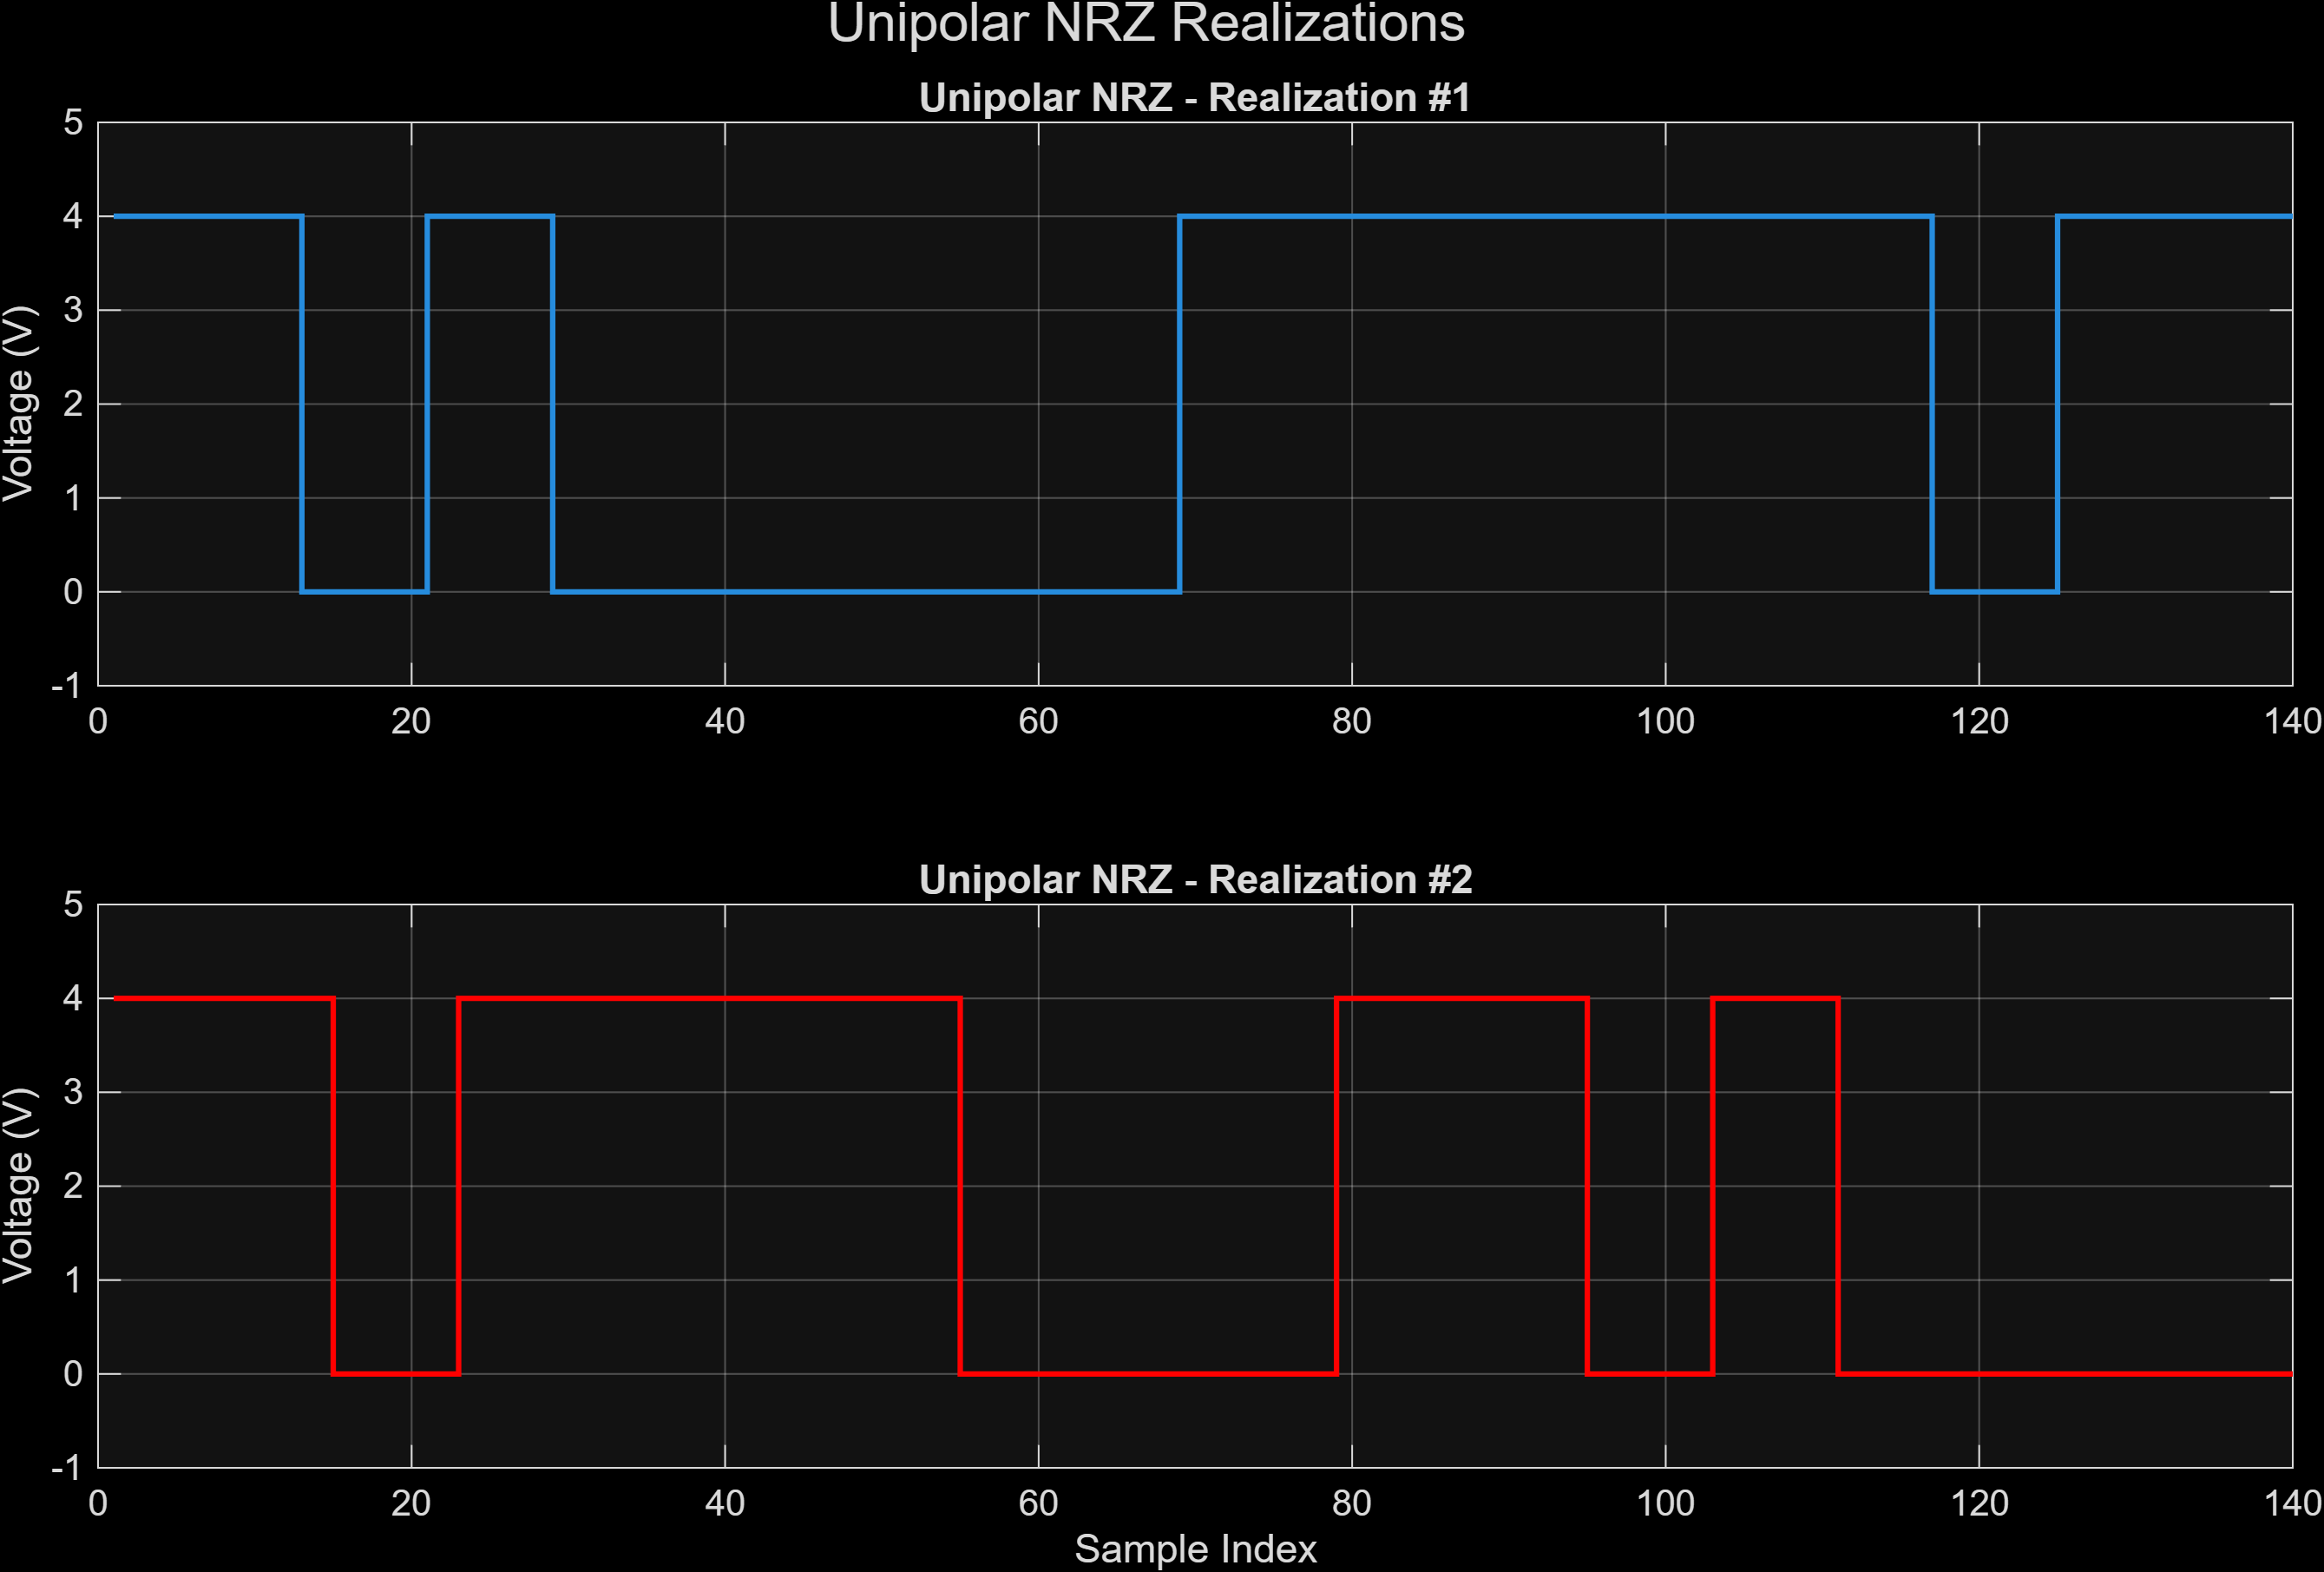
\includegraphics[width=0.75\linewidth]{Figures/Unipolar_NRZ_-_Realization_2.png}
    \caption[Realization 1 and Realzation 2 from the Unipolar Ensemble]{Realization 1 and Realzation 2 from the Unipolar Ensemble.}
    \label{fig:UNIPOLAR-ENSEMBLE}
\end{figure}

Now we can see in \ref{fig:UNIPOLAR-ENSEMBLE} the first two realizations of the
unipolar ensemble, the signal is a rectangular pulse as we expected from the
input pulse, and the amplitude maps to $0$ and $4$ as how we assigned A earlier
in the control flags. This output confirms that we succefully created the unipolar ensemble as we met the required specifications for the unipolar line code.

\begin{itemize}
    \item The amplitude of the signal is either $0$ (for bit "0") or $4$ (for bit "1").
    \item The pulse shape is rectangular, with a duration of $L$ samples per bit.
\end{itemize}